\section{Spektroskopie der Hyperfeinstruktur von Rubidium}
\subsection{Durchführung}
Bei der Messung des Hyperfein-Absorptionsspektrums befinden sich die beiden Linsen und
die Rubidiumzelle im Strahlengang.
Der Konstantanteil des Laserstroms, Modulationsamplitude und -frequenz
sind wie bei der Messung der Zeitabhängigkeit der Laserfrequenz (\autoref{sect:durchführung}).
Äußere Magnetfelder bleiben unkompensiert, weil die Zeeman-Aufspaltung der Hyperfeinstruktur im Erdmagnetfeld
mit der Linienbreite der Laserdiode nicht auflösbar ist.
Die Messung wird auf der steigenden und der fallenden Flanke der Modulationsspannung durchgeführt und
während der Messung wird die Zelle mit dem Föhn geheizt.


\subsection{Auswertung}
TODO: Fallende/Steigende Flanke, Auswertung beispielshaft für steigende flanke, fallende genau so. Spektrum für beide
\subsubsection*{Frequenzkalibrierung}  %TODO change to Berechnung der Scanrate des Lasers ?
\label{sub:scanrate}
Das Etalonspektrum und die Spannung der Lasermodulation sind in \autoref{img:etalon:fit} dargestellt.
Die Peaks des Etalonspektrums werden mit Cauchy-Kurven und einem linearen Untergrund gefittet.
\begin{equation}
    U_\text{ph}(t) = a_\text{ph} + b_\text{ph} \cdot t + \frac{A}{\pi} \frac{s}{s^2 + (t-x)^2}
\end{equation}
Dabei ist das Zentrum $x$ und der Breiteparameter $s$.
Des Weiteren wird die Spannung für die Lasermodulation mit einer Geraden gefittet.
\begin{equation}
    U_\text{L}(t) = a_\text{L} + b_\text{L} \cdot t
\end{equation}
\begin{figure}[H]
\begin{center}
    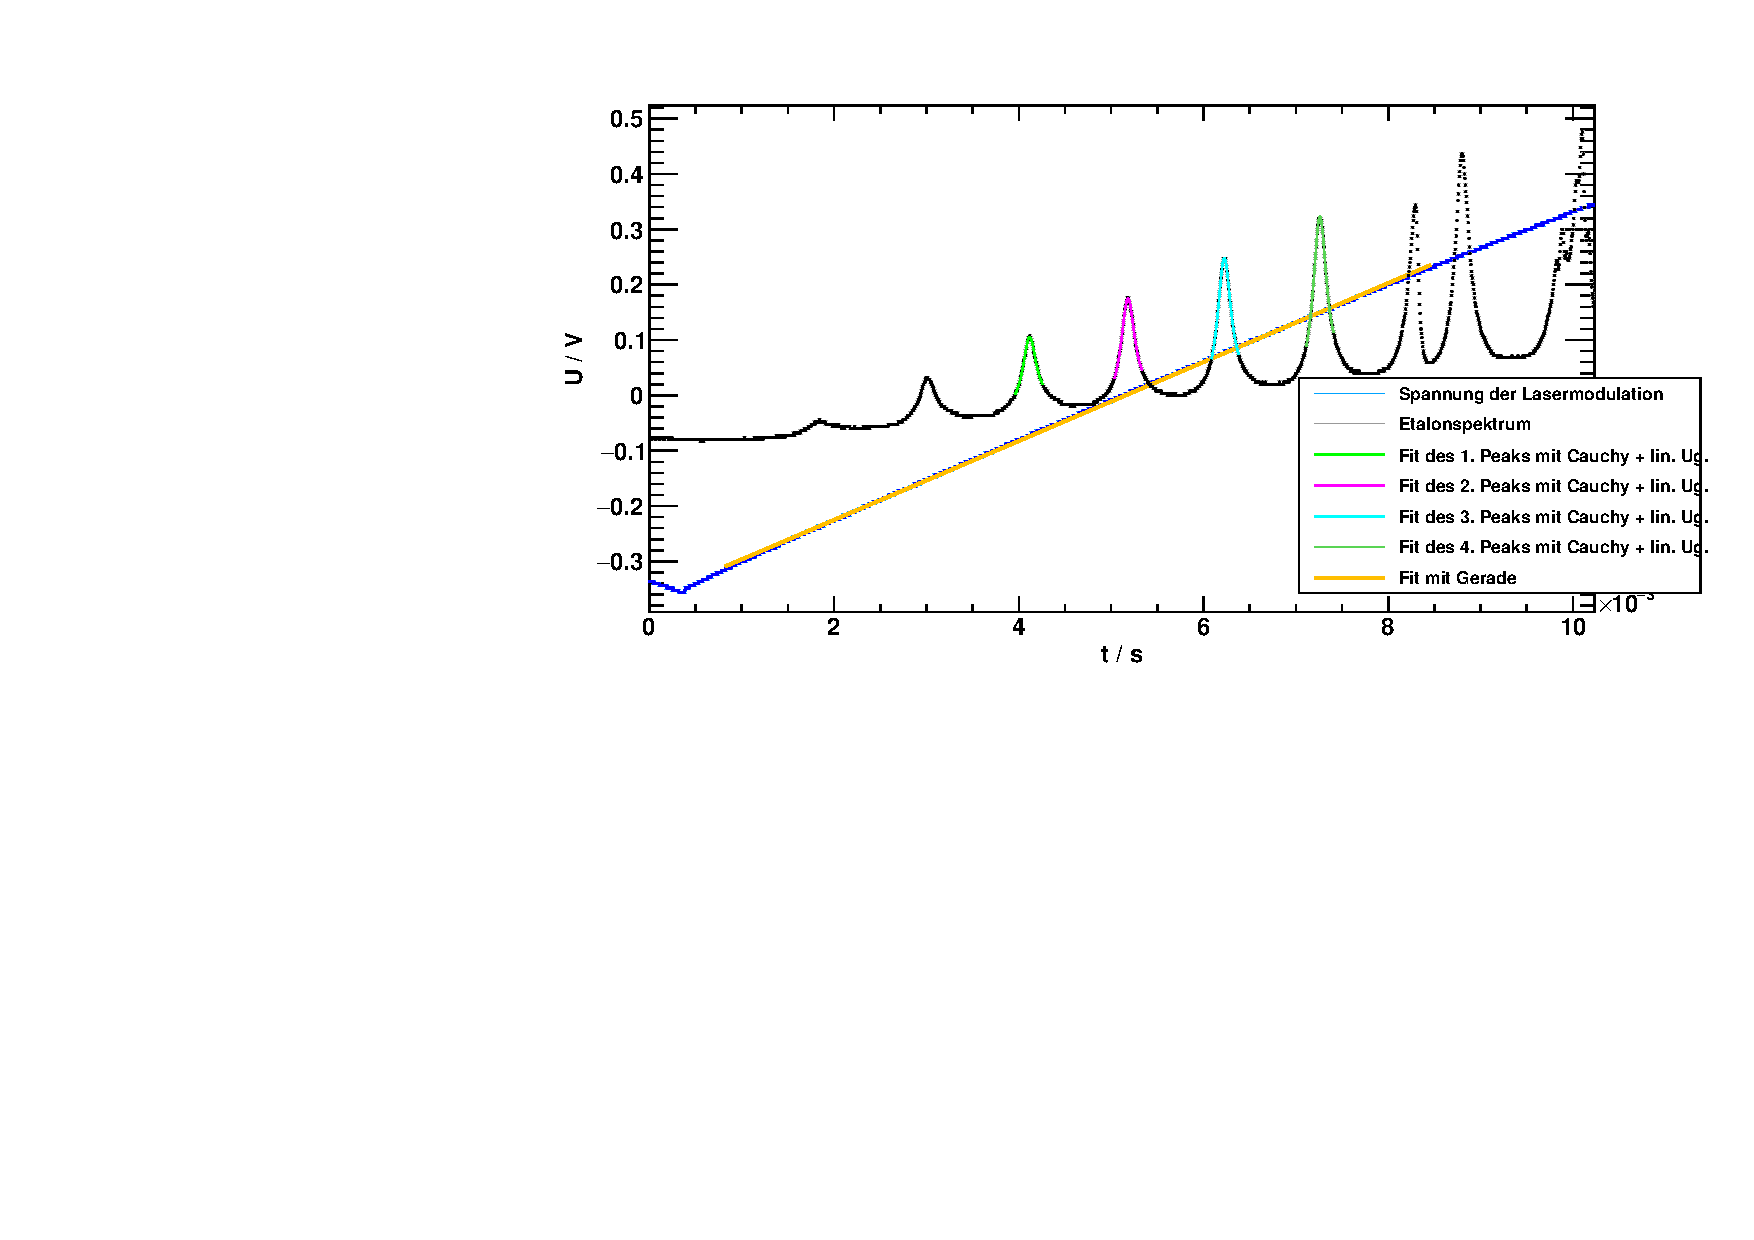
\includegraphics[width=\textwidth]{../img/part2/up-etalon_zoom_fit.pdf}
    \caption{caption.}
    \label{img:etalon:fit}
\end{center}
\end{figure}
Der Fit von $U_\text{L}$ kontrolliert, ob die Spannung für die Lasermodulation auch gerade ansteigt. Man erkennt, dass die angepasste Gerade
gut der gemessenen Spannung folgt.\\
Aus dem freien Spektralbereich des Etalons $\Delta \nu_\text{FSR} = 9924 \pm 30\,\text{MHz}$ lässt sich nun die Differenz der Laserfrequenz von den verschiedenen
Peaks bestimmen. Der erste Peak wird als Referenzpeak festgelegt. Der Frequenzabstand $\nu_i$ zwischen erstem und $i$-ten Peak lässt sich nun
folgendermaßen berechnen\footnote{Gedankenspiel zur Fehlerrechnung: Interpretiert man $2 \cdot a$ als $a + a$, so ist der Fehler im ersten Fall $2 \cdot s_a$, im zweiten
allerdings $\sqrt{2} \cdot s_a$, wenn man die Selbstkorrelation von $a$ nicht berücksichtigt. Mit $\cor(a, a) = 1$
erhält man $\sqrt{s_a^2 + s_a^2 + 2 \cdot s_a \cdot s_a \cdot \cor(a, a)} = 2 \cdot s_a$.}:
\begin{equation}
    \Delta \nu_i = i \cdot \Delta \nu_\text{FSR}, \qquad s_{\Delta \nu_i} = i \cdot s_{\Delta \nu_\text{FSR}}
\end{equation}
Die Frequenzabstände $\Delta \nu_i$ werden nun gegen die Zentren $x_i$  der
Etalonpeaks aufgetragen (\autoref{img:etalon:calibration}). Da der Fehler der Zentren der Cauchy-Funktionen viel zu gering ist, wird der Fehler
auf $\frac{1}{5}$ der Breiteparameter $s_i$ geschätzt. Die so berechneten Werte sind in \autoref{tab:etalon:calib:up} aufgelistet.
\begin{table}[H]
\caption{Zentren $x_i$ der gefitteten Cauchy-Funktionen mit abgeschätztem Fehler aus den Breiteparametern $s_i$ und Frequenzdifferenzen zum ersten Peak. }
\begin{center}
\begin{tabular}{|c|c|c|c|c|}
  \hline
  i & $x_i$ / s & $0.2 \cdot s_i$ / s & $\nu_i$ / GHz & $s_{\nu_i}$ / GHz \\ \hline
  1 & 4.117 & 0.018 & 0.00 & 0.00 \\ \hline
  2 & 5.181 & 0.018 & 9.92 & 0.03 \\ \hline
  3 & 6.225 & 0.018 & 19.85 & 0.06 \\ \hline
  4 & 7.260 & 0.018 & 29.77 & 0.09 \\ \hline
\end{tabular}
\end{center}
\label{tab:etalon:calib:up}
\end{table}

\begin{figure}[H]
\begin{center}
    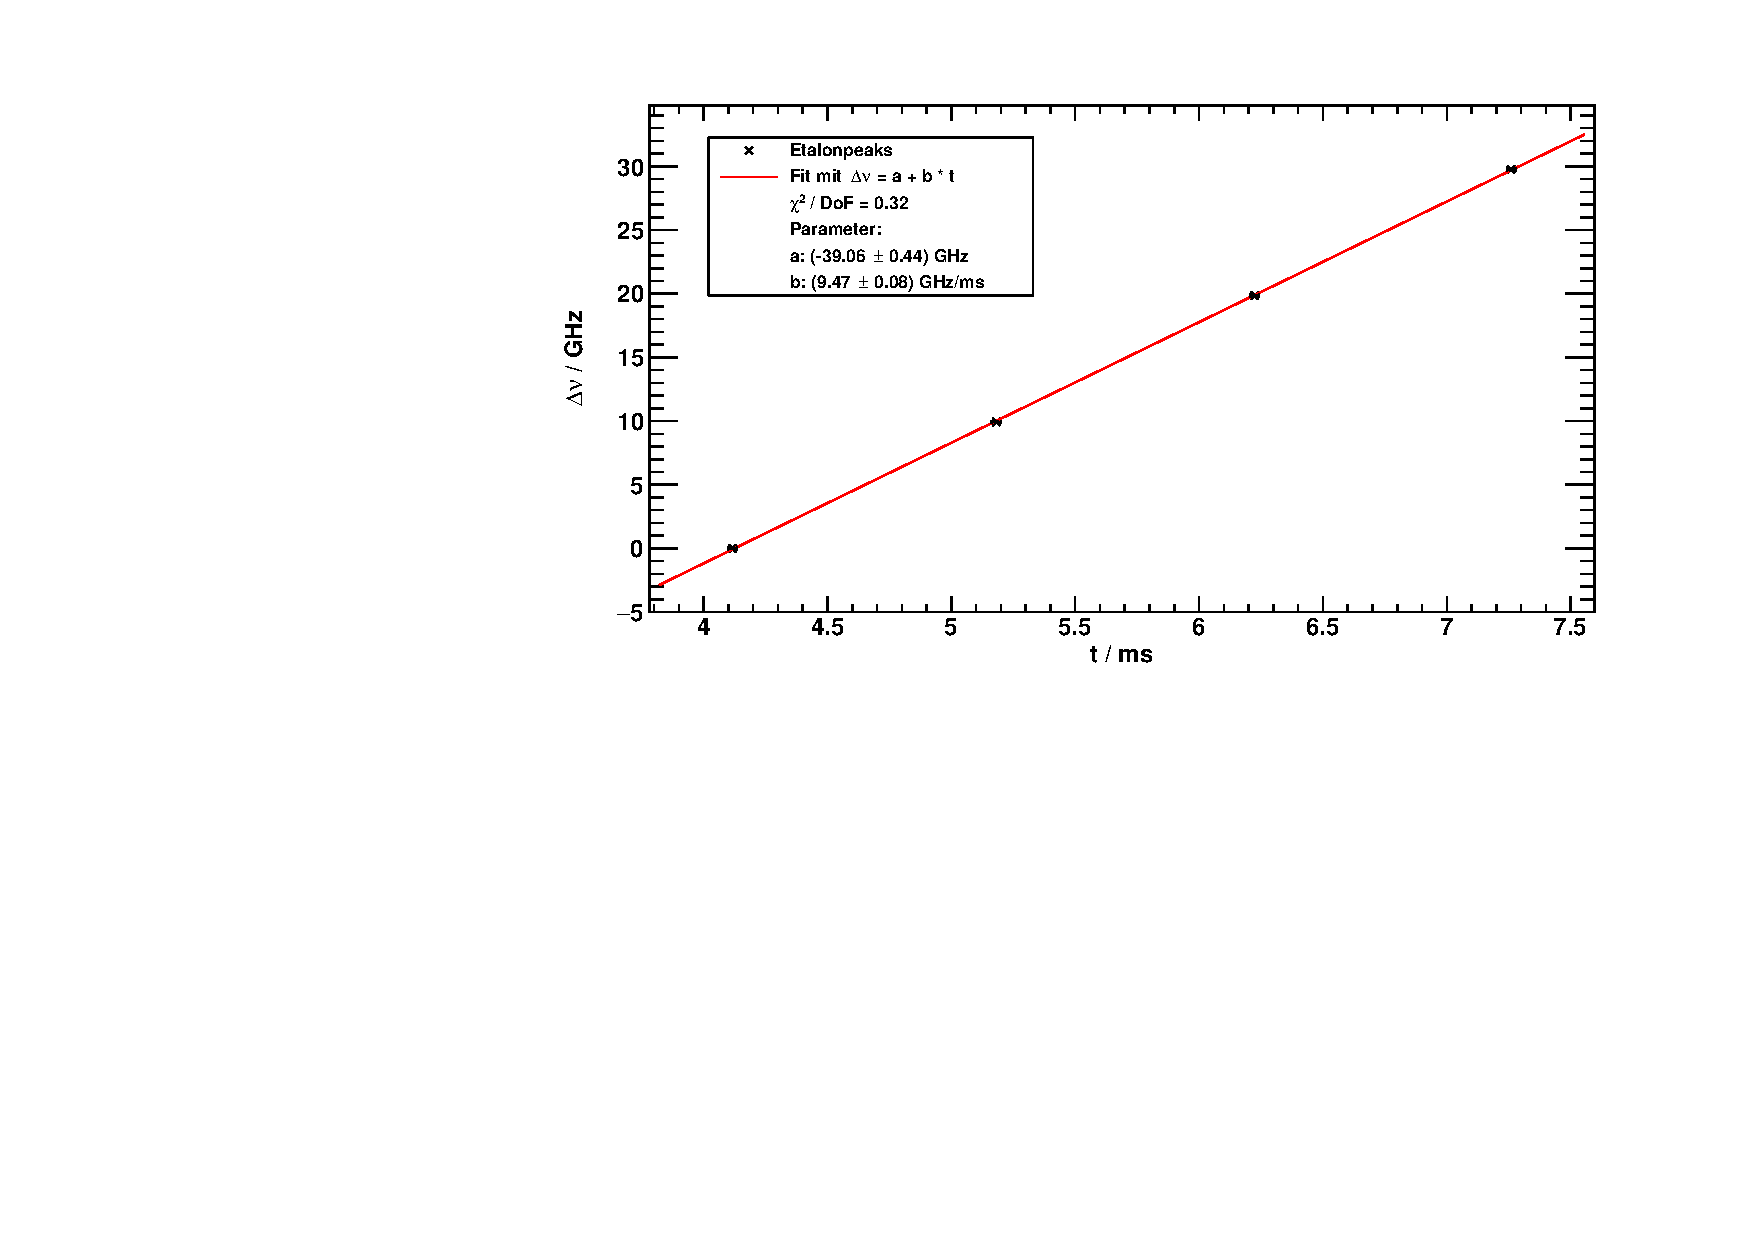
\includegraphics[width=\textwidth]{../img/part2/up-etalon_zoom-etalon_calibration.pdf}
    \caption{caption.}
    \label{img:etalon:calibration}
\end{center}
\end{figure}
Aus dem Fit mit einer Geraden
\begin{equation}
    \Delta \nu(t) = a + r \cdot t  %TODO Parameter in Plot ändern
\end{equation}
lässt sich nun die Scanrate $r$ bestimmen, mit welcher die Frequenz des Lasers pro Zeit geändert wird. Man erhält
\begin{equation}
    r = (9.40 \pm 0.02)\,\frac{\text{GHz}}{ms}\ \, .
\end{equation}

\subsubsection*{Hyperfeinstruktur-Übergänge}
Auf dem aufgenommenen Spektrum (\autoref{img:hfs:fit:up}) der Hyperfeinstruktur von Rubidium sind nur sechs der acht erwarteten
Übergänge zu erkennen (vgl. \autoref{sub:hfsspectrum}). Dies liegt daran, dass je zwei Übergänge so dicht beieinander liegen,  %TODO Ref Grundlagen
dass man sie in diesem Versuchsaufbau nicht mehr
einzeln auflösen kann. Da teilweise mehrere Übergänge dicht nebeneinander liegen, überlagern sie sich. Für die gut abtrennbaren Gruppen von
mehreren Peaks der Übergänge werden überlagerte Gauß-Funktionen mit einem linearen Untergrund zur Kurvenanpassung verwendet:
\begin{equation}
    \begin{split}
        & \gaus(x; A, \mu, \sigma) := A \cdot e^{-\frac{1}{2} \left( \frac{x-\mu}{\sigma} \right)^2} \\
        & U_\text{ph}(t) = a + b \cdot t + \sum_{i=1}^N \gaus(t; A_i, \mu_i, \sigma_i)
    \end{split}
\end{equation}
$N$ gibt an, wie viele Peaks sich überlagern.
\begin{figure}[H]
\begin{center}
    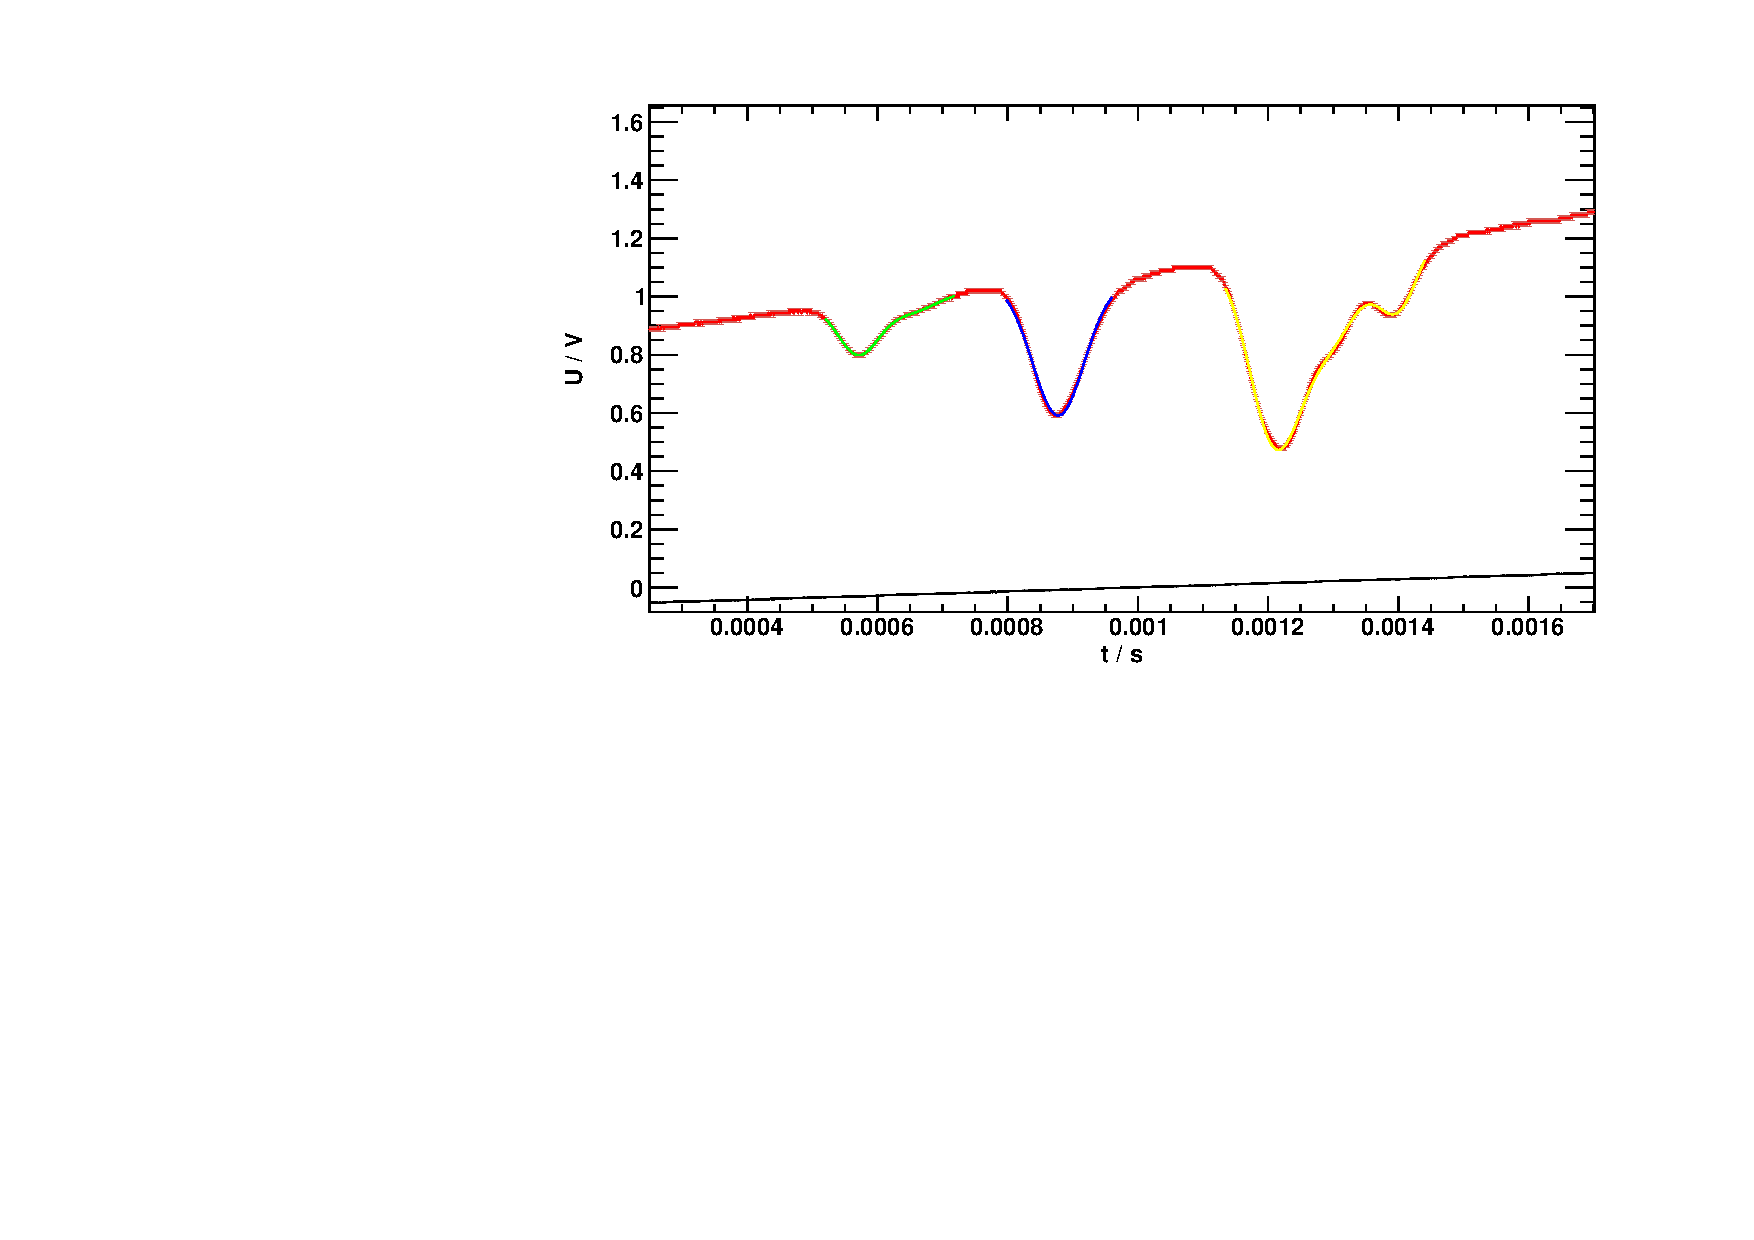
\includegraphics[width=\textwidth]{../img/part2/up-hfs_zoom_fit.pdf}  %TODO Better start params
    \caption{caption.}
    \label{img:hfs:fit:up}
\end{center}
\end{figure}
In \autoref{tab:hfs:peaks:up} sind die Erwartungswerte und Standardabweichungen der gefitteten Gauß-Funktionen aufgelistet. Da auch hier der 
Fehler auf die Erwartungswerte zu klein ist, wird der Fehler auf $\frac{1}{5}$ der Standardabweichung geschätzt.
\begin{table}[H]
\caption{Erwartungswerte $\mu_i$ und Standardabweichungen $\sigma_i$ der gefitteten Peaks des HFS-Spektrums.}
\begin{center}
\begin{tabular}{|c|c|c|c|c|}
  \hline
  Peak $i$ & $\mu_i$ / ms & $s_{\mu_i}$ / ms & $\sigma_i$ / \textmu s & $s_{\sigma_i}$ / \textmu s \\ \hline
  1 & 0.57072 & 0.00103 & 31.4 & 1.2 \\ \hline
  2 & 0.65033 & 0.01409 & 39.7 & 6.4 \\ \hline
  3 & 0.87686 & 0.00007 & 37.0 & 0.4 \\ \hline
  4 & 1.21876 & 0.00009 & 53.2 & 0.6 \\ \hline
  5 & 1.30931 & 0.00022 & 23.7 & 0.3 \\ \hline
  6 & 1.38975 & 0.00024 & 43.5 & 0.9 \\ \hline
\end{tabular}
\end{center}
\label{tab:hfs:peaks:up}
\end{table}


\subsubsection*{Berechnung des Spektrums}
Da die Differenzen der einzelnen Hyperfeinniveaus in der Größenordnung von $10^9$\,Hz liegen und die absoluten Frequenzen bei $101 {14}$\,Hz, 
wird verzichtet, die absoluten Frequenzen auszurechnen. Der Peak mit der größten Amplitude (Peak 4) wird als Referenz gesetzt. Von ihm aus werden 
die Differenzen zu den anderen Peaks berechnet. Dazu wird die oben (\autoref{sub:scanrate}) berechnete Scanrate $r$ des Lasers benötigt.
Die Differenzen der Frequenzen $\Delta \nu_i$ zwischen viertem und $i$-tem Peak berechnen sich nun mit
\begin{equation}
    \Delta \nu_i = r \cdot \left( \mu_i - \mu_4 \right), 
    \qquad s_{\Delta \nu_i} = \Delta \nu_i \sqrt{ \left( \frac{s_r}{r} \right)^2 + \frac{s_{\mu_i}^2 + s_{\mu_4}^2}{ \left( \mu_i - \mu_4 \right)^2 }} \ \, .
\end{equation}
Mit dieser Formel für den Fehler von $\Delta \nu_i$ ist der Fehler auf $\Delta \nu_4$ nicht definiert, da eine Division durch Null stattfindet.
Um doch einen Fehler zu bekommen, wird angenommen, dass de keinen Fehler hat. Man erhält mit Gauß'scher Fehlerfortpflanzung
\begin{equation}
    s_{\Delta \nu_4} = r \cdot s_{\mu_4} \ \, .
\end{equation}
Um die theoretischen Werte sinnvoll mit den gemessenen Werten zu vergleichen, müssen die theoretischen Differenzen der Frequenz den gleichen 
Übergang als Referenz benutzen. Dies erreicht man, wenn die Differenz der Frequenz des Referenzübergangs von allen Differenzen abgezogen wird.
In \autoref{tab:hfs:spectrum} sind die theoretischen und experimentell bestimmten (für steigende und fallende Flanke) Spektren aufgelistet.   
\begin{table}[H]
\caption{Theoretisches und experimentell bestimmtes (steigende und fallende Flanke) Hyperfeinstrukturspektrum von Rubidium.}
\begin{center}
\begin{tabular}{|c|c|c|c|c|c|}
  \hline
  Übergang & $\Delta \nu^\text{theo}$ / GHz & $\Delta \nu^\text{exp}_\text{up}$ / GHz & $s_{\Delta \nu^\text{exp}_\text{up}}$ / GHz & $\Delta \nu^\text{exp}_\text{down}$ / GHz & $s_{\Delta \nu^\text{exp}_\text{down}}$ / GHz \\ \hline
  \rb{87}, F:2-1 & -4.81 & -4.86 & 0.12 & -4.95 & 0.10 \\ \hline
  \rb{87}, F:2-2 & -3.99 & -4.10 & 0.09 & -4.24 & 0.10 \\ \hline
  \rb{85}, F:3-2, 3-3 & -3.04 & -3.24 & 0.13 & -3.25 & 0.12 \\ \hline
  \rb{85}, F:2-2, 2-3 & 0.00 & 0.00 & 0.07 & -0.00 & 0.07 \\ \hline
  \rb{87}, F:1-1 & 2.02 & 2.15 & 0.10 & 2.01 & 0.09 \\ \hline
  \rb{87}, F:1-2 & 2.84 & 2.90 & 0.09 & 2.85 & 0.10 \\ \hline
\end{tabular}
\end{center}
\label{tab:hfs:spectrum}
\end{table}

Zur Überprüfung, wie gut die theoretischen Daten mit den gemessenen übereinstimmen, können sie gegeneinander aufgetragen werden 
( \autoref{img:hfs:spectrum:up} für die steigende und \autoref{img:hfs:spectrum:down} für die fallende Flanke). Es sollte sich 
eine Gerade mit Steigung 1 und Achsenabschnitt 0 ergeben.

\begin{figure}[H]
\begin{center}
    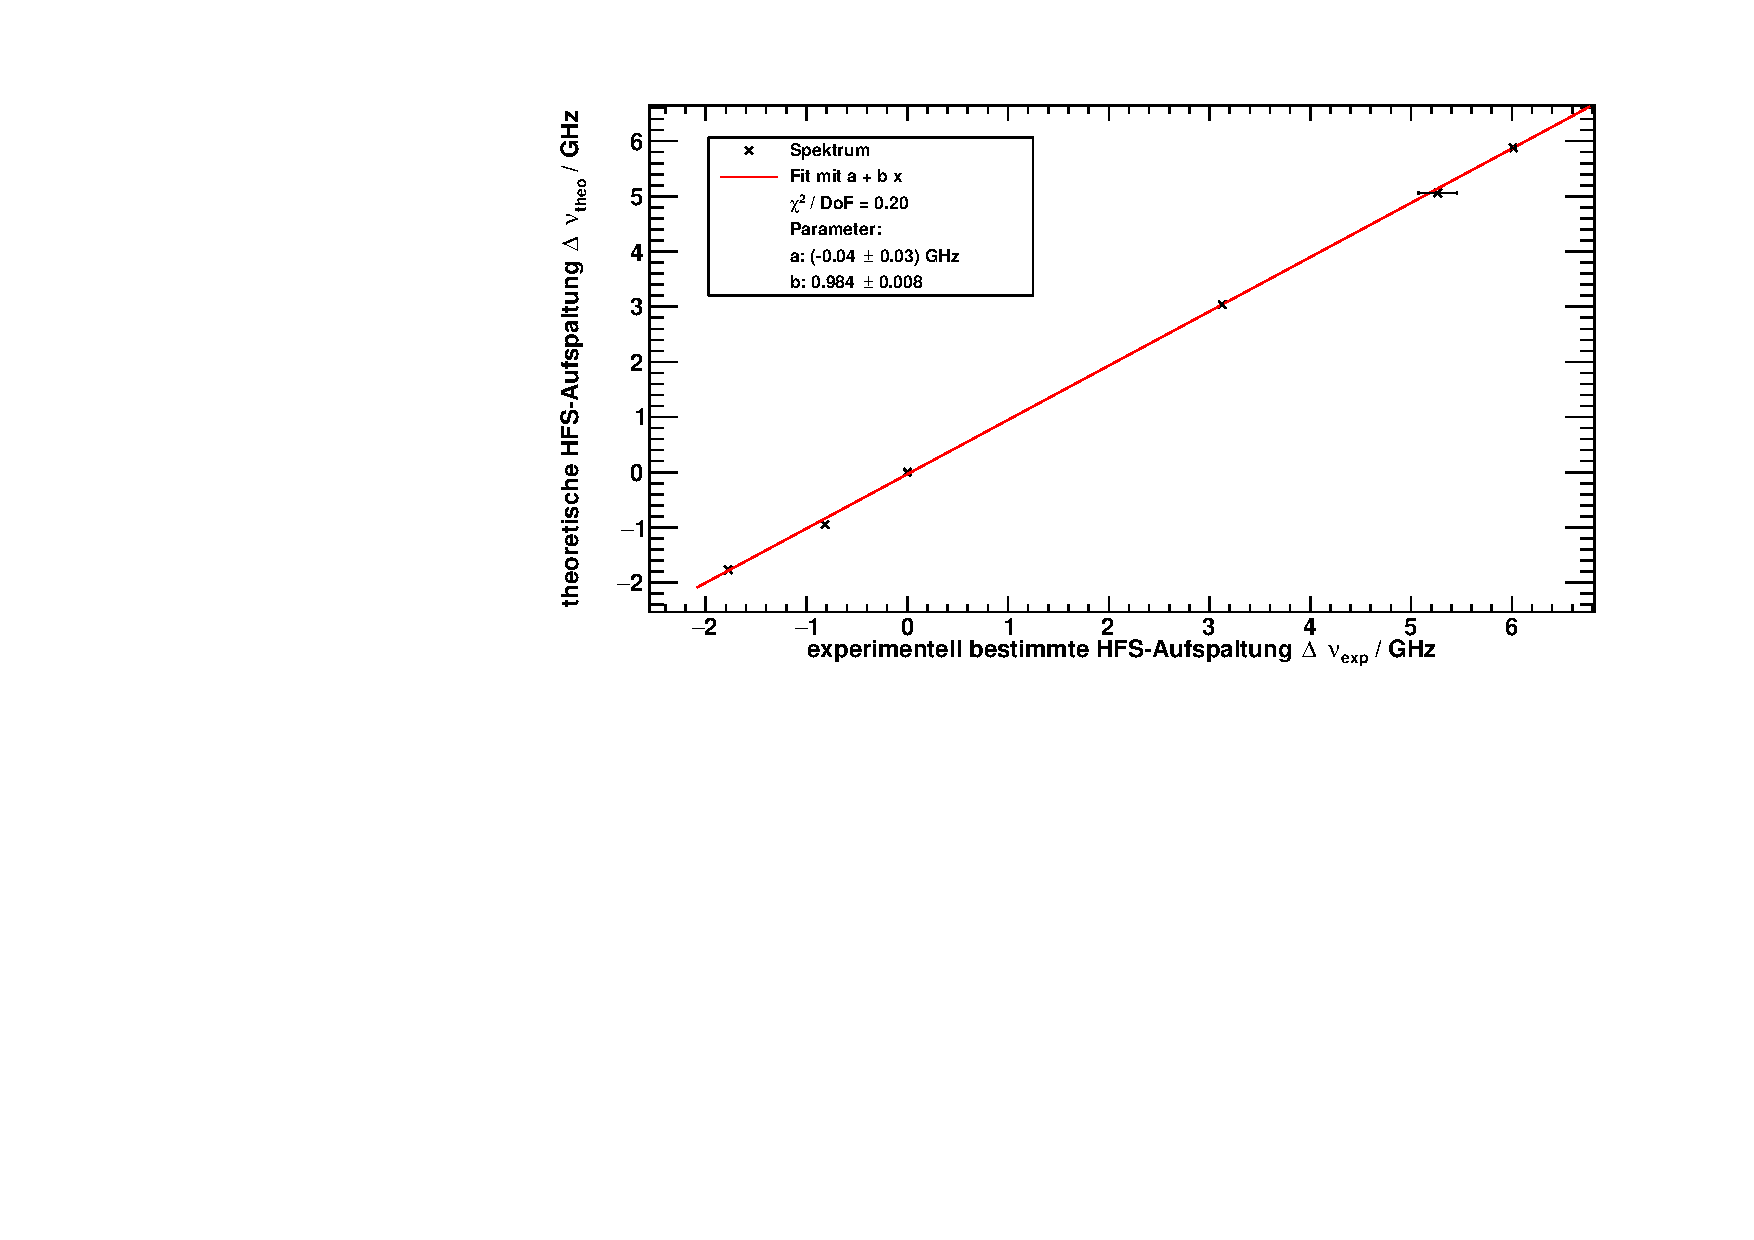
\includegraphics[width=\textwidth]{../img/part2/up-spectrum.pdf}
    \caption{caption.}
    \label{img:hfs:spectrum:up}
\end{center}
\end{figure}

\begin{figure}[H]
\begin{center}
    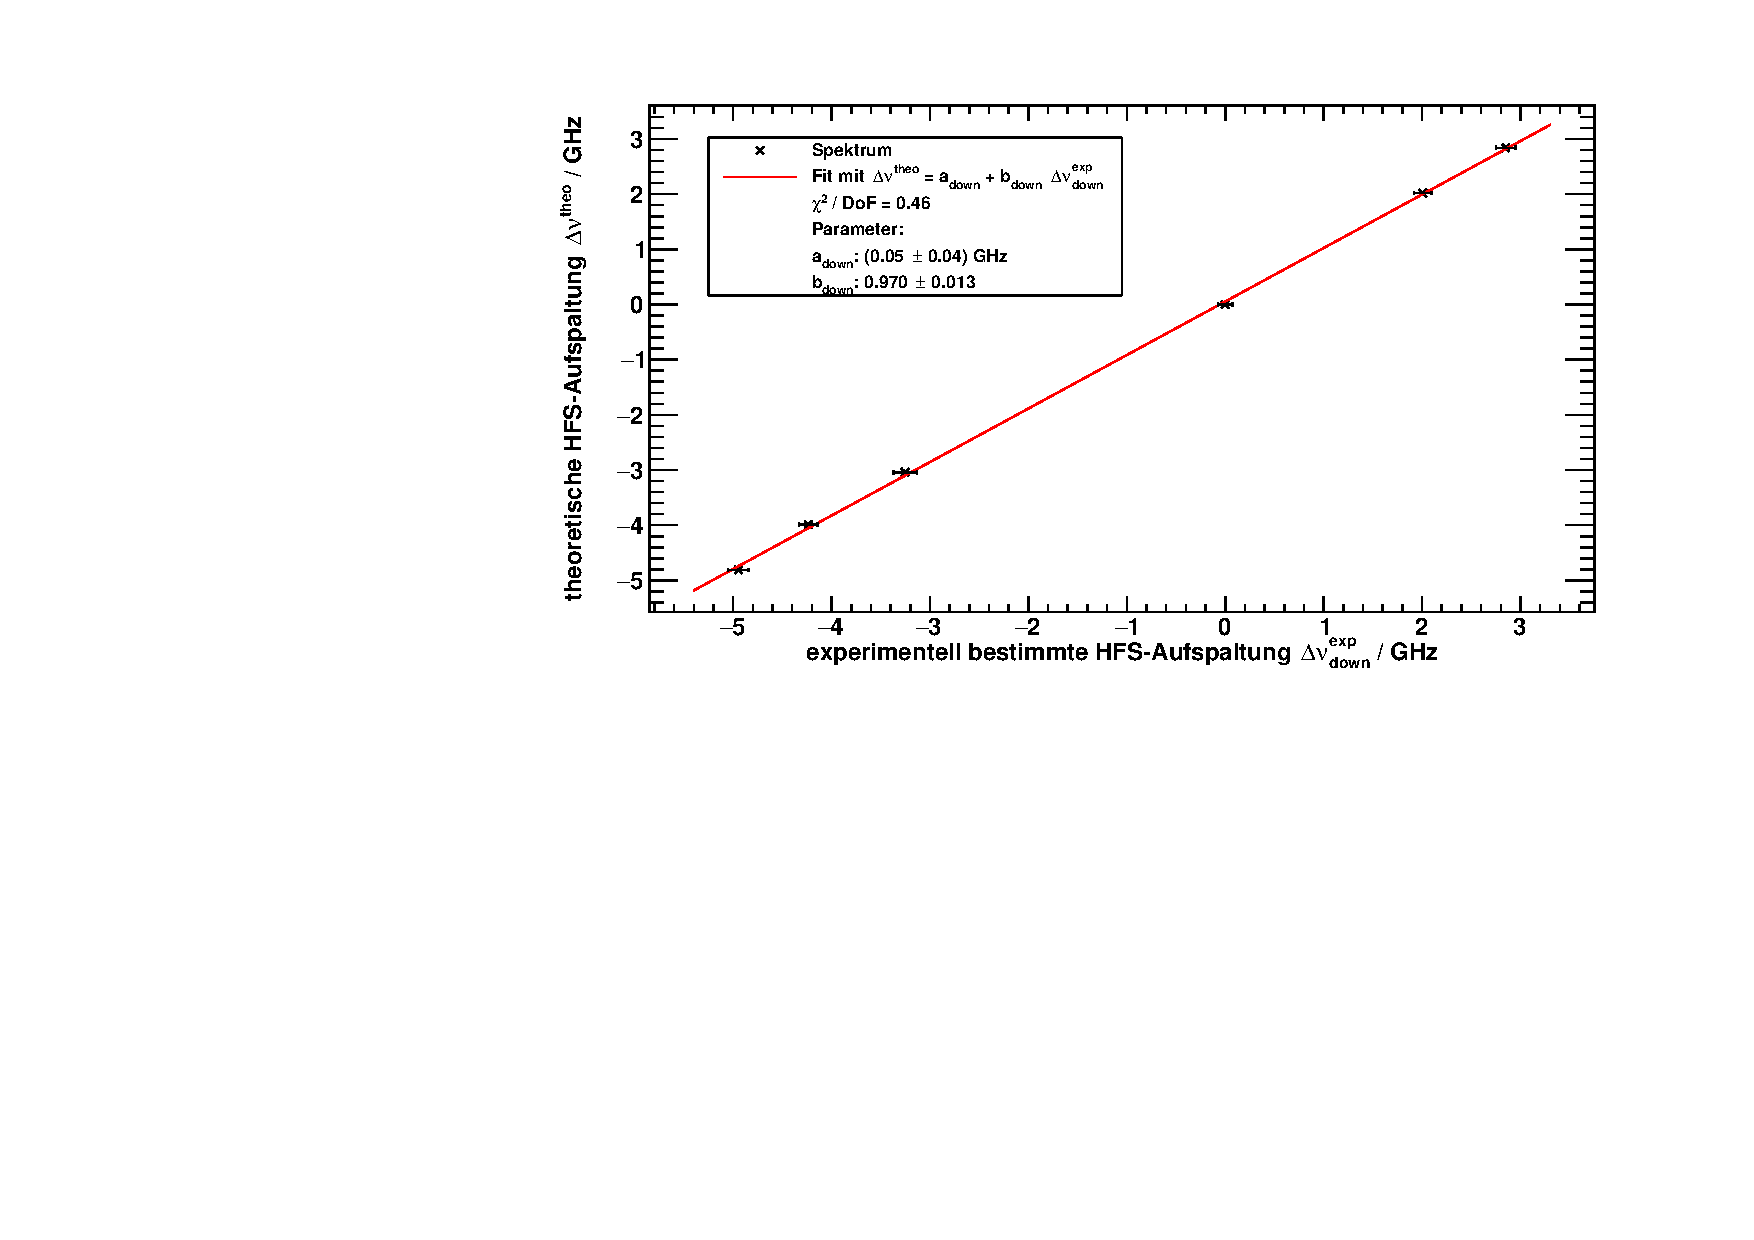
\includegraphics[width=\textwidth]{../img/part2/down-spectrum.pdf}
    \caption{caption.}
    \label{img:hfs:spectrum:down}
\end{center}
\end{figure}
Die Achsenabschnitte 
\begin{equation}
    a_\text{up} = (-0.01 \pm 0.04)\,\text{GHz} \quad \text{und} \quad a_\text{down} = (0.04 \pm 0.05)\,\text{GHz}
\end{equation}
und Steigungen
\begin{equation}
    b_\text{up} = (0.973 \pm 0.013) \quad \text{und} \quad b_\text{down} = (0.970 \pm 0.013)
\end{equation}
bestätigen die Übereinstimmung mit den theoretischen Werten innerhalb eines maximal 3-\textsigma-Intervalls.

\subsubsection*{Berechnung der Intervallkonstanten $A$}
Für die Berechnung der Intervallkonstanten $A$ wird für jeden Übergang das gewichtete Mittel der Frequenzendifferenz von steigender und fallender 
Flanke gebildet (\autoref{tab:hfs:spectrum:avg}).
\begin{table}[H]
\caption{Theoretisches und aus den experimentellen Daten gemitteltes Hyperfeinstrukturspektrum von Rubidium.}
\begin{center}
\begin{tabular}{|c|c|c|c|}
  \hline
  Übergang & $\Delta \nu^\text{theo}$ / GHz & $\Delta \nu^\text{exp}_\text{avg}$ / GHz & $s_{\Delta \nu^\text{exp}_\text{avg}}$ / GHz \\ \hline
  \rb{87}, F:2-1 & -4.81 & -4.907 & 0.077 \\ \hline
  \rb{87}, F:2-2 & -3.99 & -4.162 & 0.065 \\ \hline
  \rb{85}, F:3-2, 3-3 & -3.04 & -3.246 & 0.087 \\ \hline
  \rb{85}, F:2-2, 2-3 & 0.00 & 0.000 & 0.051 \\ \hline
  \rb{87}, F:1-1 & 2.02 & 2.065 & 0.067 \\ \hline
  \rb{87}, F:1-2 & 2.84 & 2.876 & 0.069 \\ \hline
\end{tabular}
\end{center}
\label{tab:hfs:spectrum:avg}
\end{table}

Für die Berechnung der Intervallkonstanten wird die 
Beschreibung Berechnung $\Delta \nu_F$ (2 Möglichkeiten, Differenz zu bilden, gewichtetes Mittel) \\
Berechnung A für S und P
\begin{equation}
    A = \Delta \nu \cdot \frac{h}{F + 1}, \qquad s_A = s_{\Delta \nu} \cdot \frac{h}{F + 1}
\end{equation}
\begin{table}[H]
\caption{Errechnete HFS-Intervallkonstanten $A$ für die zwei untersten Feinstrukturniveus von \rb{87}.}
\begin{center}
\begin{tabular}{|c|c|c|c|}
  \hline
  Feinstruktur & $A^\text{Lit.}$ / \textmu eV & $A^\text{exp}$ / \textmu eV & $s_{A^\text{exp}}$ / \textmu eV \\ \hline
  ${}^2\text{S}_{1/2}$ & 14.13 & 14.49 & 0.14 \\ \hline
  ${}^2\text{P}_{1/2}$ & 1.692 & 1.61 & 0.14 \\ \hline
\end{tabular}
\end{center}
\label{tab:hfs:intervalconsts}
\end{table}
